\section{Sample Model}
% sample model: integration equation

To make every explanation in upcoming sections easy to understand,  a sample model of a circuit at the architectural level will be used. The model that has been chosen is circuit that solve the following equation :

\begin{equation}
    \citeequation{y\prime\prime + 3xy\prime +3y}{main}\label{diffeq}
\end{equation}

\begin{figure}[ht]
    \centering
    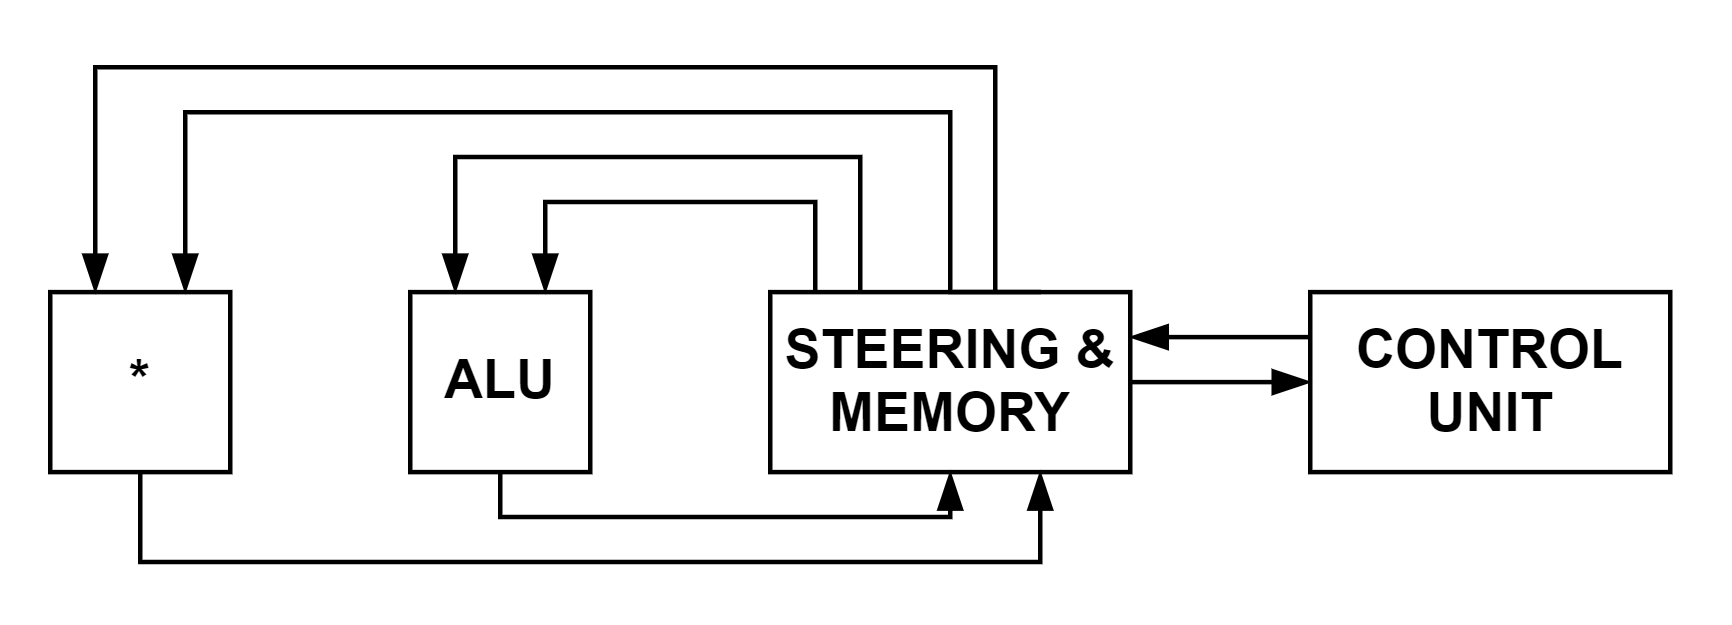
\includegraphics[width=0.35\textwidth]{Example_of_structural_view_at_the_architectural_level}
    \caption{Example of structural view at the architectural level. \cite{main}}
    \label{Example_of_structural_view_at_the_architectural_level}
\end{figure}

The structural view of the model at architectural level is shown in ``Fig. \ref{Example_of_structural_view_at_the_architectural_level}" and the behavioural view of the model at architectural level can be written in HDL as follows \cite{main}:

\begin{lstlisting}
diffeq {
    read(x, y, u, dx, a);
    repeat {
        xl = x + dx ;
        ul = u - ( 3*x*u*dx ) - ( 3*y*dx );
        yl = y + u*dx;
        c = xl < a;
        x = xl ; u = ul ; y = yl;
        }
    intil ( c );
    write ( y );
}
\end{lstlisting}

From the behaviour model, we could see that the solution involving iteration of set of operations. The set of operation in each iteration (within the repeat function) can be broke into 11 simple operation and can be modelled using data-flow graph as shown in ``Fig. \ref{Example_of_a_data-flow_graph}" to represent the abstract model of the solution at architectural level in terms of tasks and their dependencies \cite{main}. The task could be \textit{No-Operation} (NOPs) if the task does not involve any operation or task that can be executed instantaneously without side effect. 

\begin{figure}[ht]
    \centering
    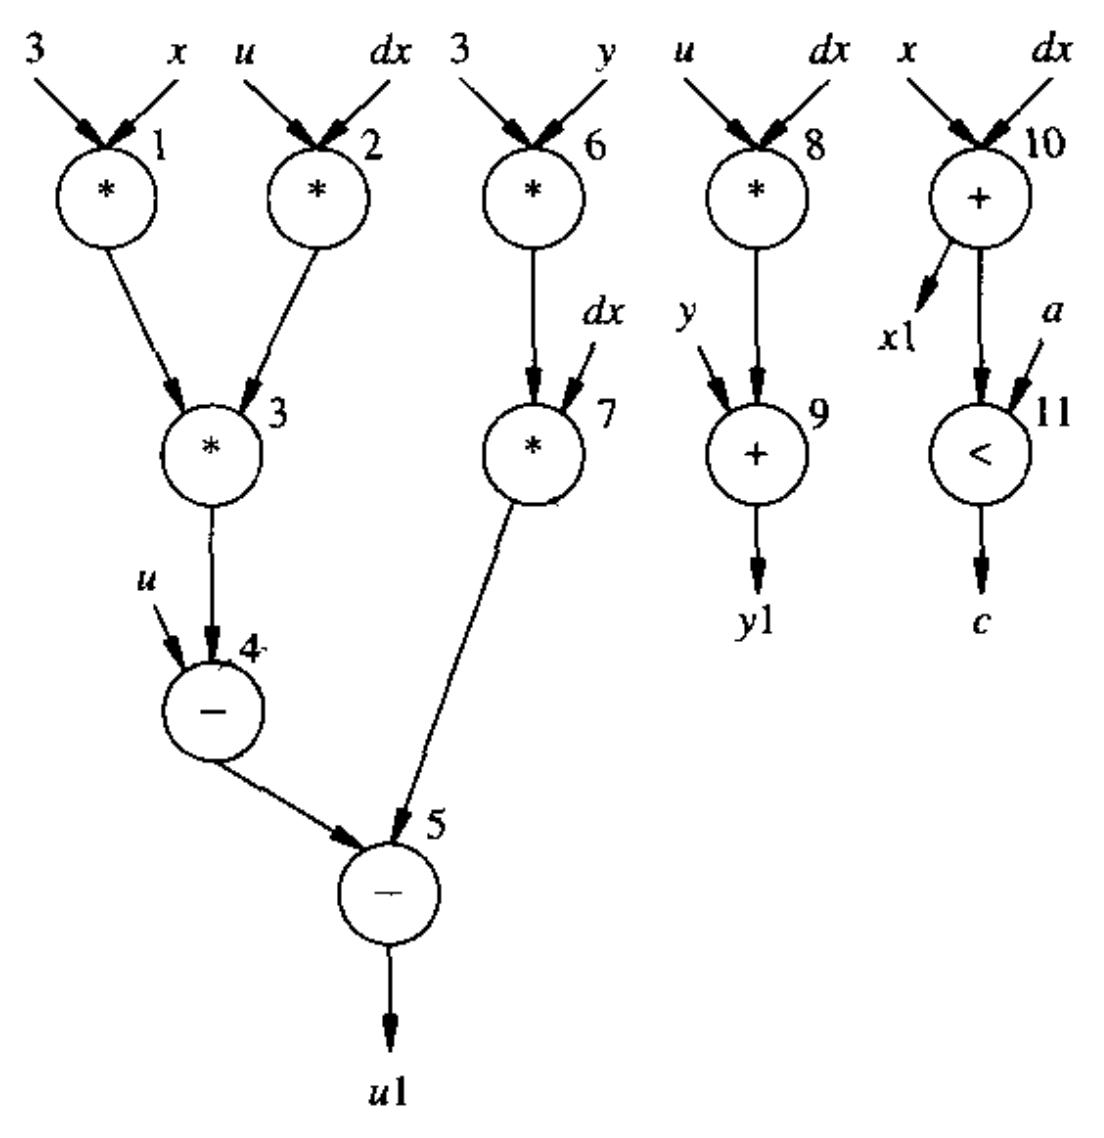
\includegraphics[width=0.35\textwidth]{Example_of_a_data-flow_graph}
    \caption{Example of a data-flow graph. \cite{main}}
    \label{Example_of_a_data-flow_graph}
\end{figure}

Regrading the branching and iteration, the control-flow information can be modelled using a control-flow graph. According to \cite{main}---``Many models have been proposed to represent control data-flow graphs (CDFGs)". One of the main CDFG that will be intensively used in this paper is sequencing graph,  $G_{s}(V, E)$, as illustrate in``Fig. \ref{Example_of_ a_sequencing_graph}" that represent the circuit model where $V$ is the vertex set, $ V = \{v_{i}; i = 0, 1.. . . , n\}$ and $E$ is the set of edges, $ E = \{(v_{i}, v_{j}); i, j = 0, 1, ... , n\} $. 
Based on the ``Fig. \ref{Example_of_ a_sequencing_graph}", the graph has two properties :

\begin{itemize}
    \item Polar : The source and sink vertices are labelled with $v_{0}$ and $v_{n}$ representing the start and the last task.Both are NOPs.
    \item Acyclic : No iteration or loop because the iteration and branching are modelled outside the graph.
\end{itemize}

\begin{figure}[ht]
    \centering
    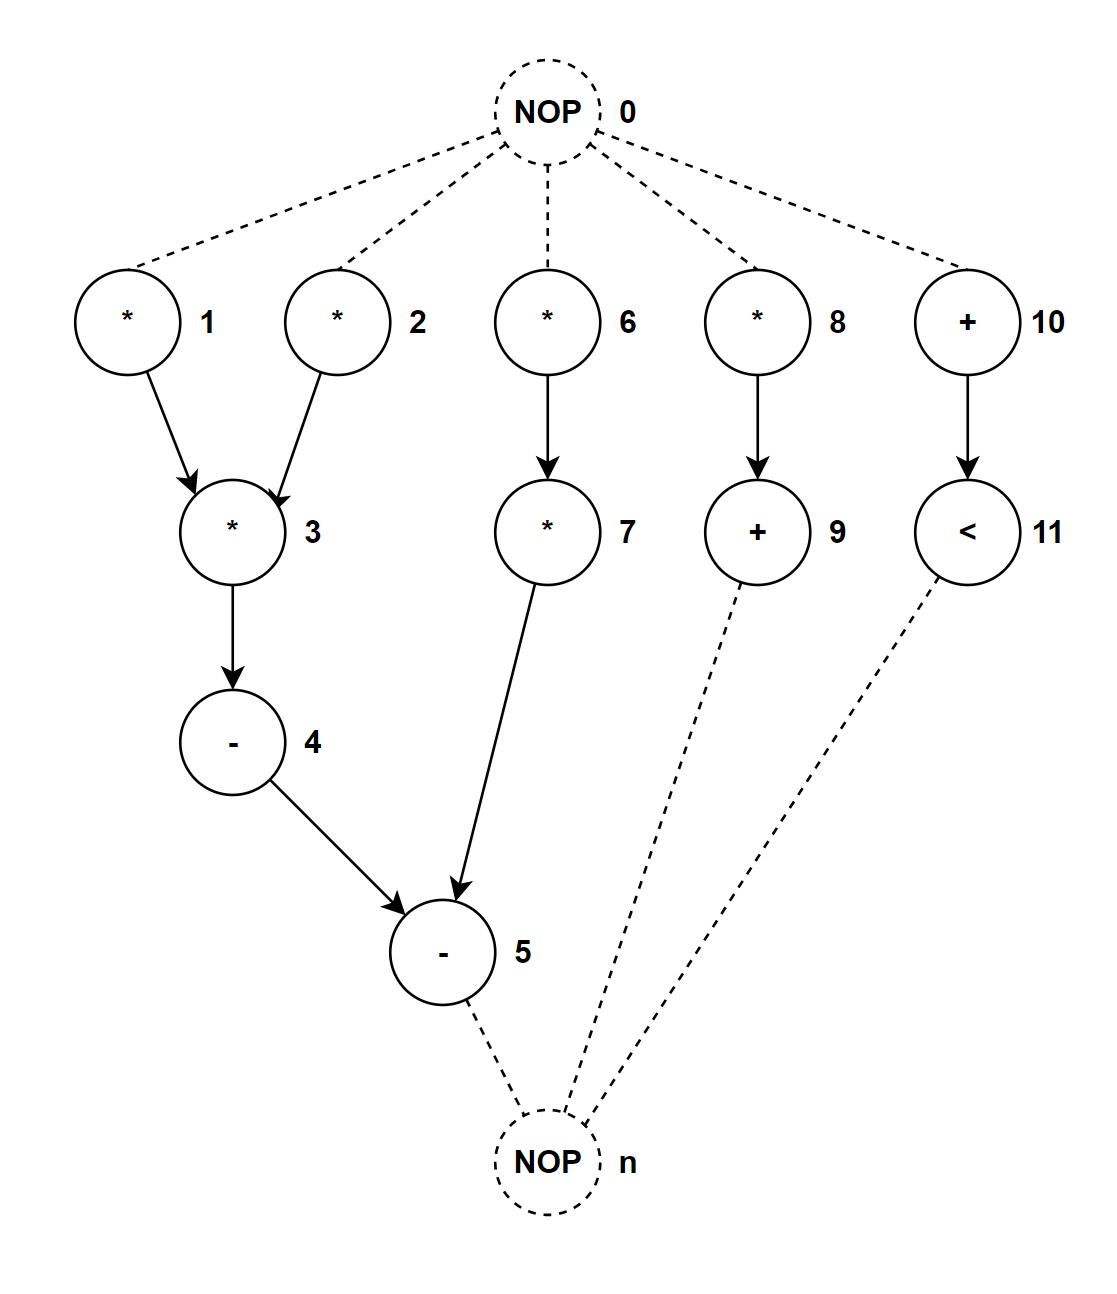
\includegraphics[width=0.35\textwidth]{Example_of_ a_sequencing_graph}
    \caption{Example of a sequencing graph. \cite{main}}
    \label{Example_of_ a_sequencing_graph}
\end{figure}



As stated, the iteration and branching are modelled outside this graph means that path in the graph not representing alternative but concurrent streams of operation \cite{main}. But it does not mean that the sequencing graph cannot model loop and branching. They do, but in a hierarchical way.


After a solution or the circuit have been model, the specification should be further described. The model specification will be explained more in the next sub topic.